\newcommand{\likertbarchart}[6]{%
  \begin{figure}[H]
    \centering
    \begin{tikzpicture}
      \begin{axis}[
        width=\textwidth / 2,
        xbar,
        xmin=0,
        xmax=12,
        ticklabel style={font=\small},
        label style={font=\small},
        nodes near coords style={font=\small},
        bar width=20,
        nodes near coords,
        xlabel={Number of mentions},
        grid=both,
        grid style={line width=.1pt, draw=gray!10},
        major grid style={line width=.2pt,draw=gray!50},
        minor x tick num=1,
        ytick=data,
        yticklabels={Trifft zu, Trifft eher zu, Trifft eher nicht zu, Trifft nicht zu},
      ]
        \addplot[black,fill=blue!30!white] coordinates{ (#3,4) (#4,3) (#5,2) (#6,1)};
      \end{axis}
    \end{tikzpicture}
    \caption{#1}
    \label{#2}
  \end{figure}
}
\chapter{User Test Results}
\label{chap:app_user_test_results}
To minimize linguistic misunderstandings (especially with text answers), we
decided to conduct the questionnaire of the user test in the native language of
the participants (German). This appendix, therefore, lists all questions and
answers in the original language.

\section{Questions about Sequences} % (fold)
\label{sec:Questions about Sequences}
\textit{Note:} Initially, the Sequence library was called Sequence framework.
The questions, therefore, use the old name.

\subsection*{Question 1}
\label{sub:ut_q1}
Mir war sofort klar, was die Parameter des Sequenz-Konstruktors bedeuten und wie ich sie definieren muss.
\likertbarchart
  {Answers to question 1}
  {fig:app_usertest_q1}
  {8}{5}{0}{0}

\subsection*{Question 2}
\label{sub:ut_q2}
Ich brauche Funktionen wie map, filter, take, reduce häufig wenn ich mit Listen, Arrays oder Ähnlichem arbeite.
\likertbarchart
  {Answers to question 2}
  {fig:app_usertest_q2}
  {9}{3}{1}{0}
% section Questions about Sequences (end)

\subsection*{Question 3}
\label{sub:ut_q3}
Die Codebeispiele in der JSDoc von take, uncons usw. waren hilfreich. 
\likertbarchart
  {Answers to question 3}
  {fig:app_usertest_q3}
  {6}{5}{1}{1}

\subsection*{Question 4}
\label{sub:ut_q4}
Ich kann mir vorstellen, in einem zukünftigen Projekt das Sequenzframework zu verwenden.
\likertbarchart
  {Answers to question 4}
  {fig:app_usertest_q4}
  {6}{4}{2}{1}

\subsection*{Question 5}
\label{sub:ut_q5}
Diese Funktionen brauche ich sonst noch oft im Zusammenhang mit Listen.

\textit{Note:} This multi select question allows us to discover missing
operators in the Sequence library.
  \begin{figure}[H]
    \centering
    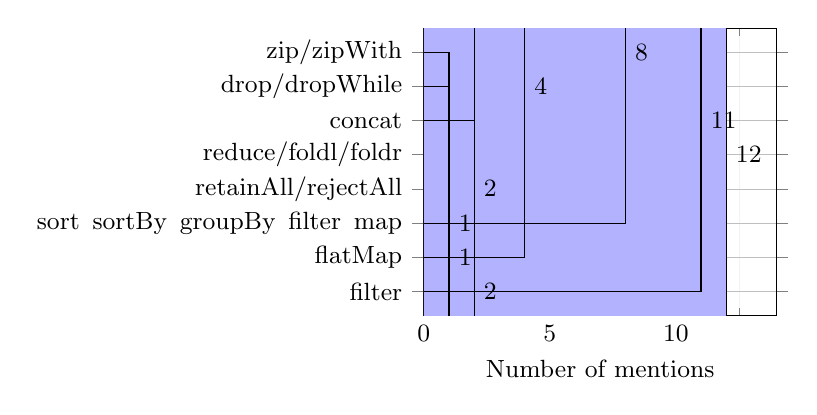
\begin{tikzpicture}
      \begin{axis}[
        width=\textwidth / 2,
        xbar,
        xmin=0,
        xmax=14,
        ticklabel style={font=\small},
        label style={font=\small},
        nodes near coords style={font=\small},
        bar width=10,
        nodes near coords,
        xlabel={Number of mentions},
        grid=both,
        grid style={line width=.1pt, draw=gray!10},
        major grid style={line width=.2pt,draw=gray!50},
        minor x tick num=1,
        ytick=data,
        yticklabels={zip/zipWith, drop/dropWhile, concat, reduce/foldl/foldr, retainAll/rejectAll, sort\, sortBy\, groupBy\, filter\, map, flatMap, filter },
      ]
        \addplot[black,fill=blue!30!white] coordinates{ (8,8) (4,7) (11,6) (12,5) (2,4) (1,3) (1,2) (2,1) };
      \end{axis}
    \end{tikzpicture}
    \caption{Answers to question 5}
    \label{fig:app_usertest_q5}
  \end{figure}
\subsection*{Question 6}
\label{sub:ut_q6}
Ich finde es sinnvoll, das Sequenzframework über einen Namen (im Test `\_`) zu importieren, um bessere IDE Unterstützung zu erhalten.
\likertbarchart
  {Answers to question 6}
  {fig:app_usertest_q6}
  {8}{4}{1}{0}

\subsection*{Question 7}
\label{sub:ut_q7}
Was gefiel Ihnen im Zusammenhang mit Sequenzen, was weniger?
\begin{table}[H]
  \centering
  \begin{tabularx}{\textwidth}{| X |} \hline
   Der funktionale Stil, aber das liegt bloss an persoenlicher Vorliebe. Prinzipiell eine gute Idee, aber die Funktionen sind so simpel, dass ich das lieber selber schreibe, als dafuer ein Framework zu lernen. \\ \hline 
   Sehr schnell verständlich wie es aufgebaut und somit zu verwenden ist. So machen auch Mathematische Funktionen schon fast Spass :D \\ \hline 
   Dank der Beschreibung ab Zeile 60 war mir sofort klar, was eine Sequenz ist und was man im Konstruktor angeben muss. Das Beispiel JSDoc ist mir erst aufgefallen, als ich mit der Aufgabe fertig war und den Fragebogen gestartet habe. Ein Beispiel wäre aber sicher von Anfang an hilfreich gewesen. Ich denke so ein SequenzFramework kann viel Arbeit abnehmen und auch den Code lesbarer machen. Allerdings hätte ich das Sequenzframework mit einem anderen Namen importiert anstatt mit \_. \\ \hline
   hat jetzt nicht wirklich den anreiz, da es auch mit vanilla js machbar ist und nicht wirklich schwer zu implementieren ist \\ \hline 
   Die Art wie mit diesen Sequenzen gearbeitet werden kann und die gebotene Funktionalität, gefällt mir gut. Hatte einzig etwas mühe, JSDocs in Verbindung mit dem Curring zu lesen. Die Beispiele waren da jeweils deutlich hilfricher, als der angezeigte Typ der Funktoin (z.B. bei \_.map) \\ \hline 
   Mir gefiel den Einstieg und die Dokumentation. Ich habe eigentlich nichts was mir nicht so gefallen hat. \\ \hline 
   +Ähnlichkeit in der Anwendung zu Haskell und anderen funktionalen Sprachen \\ \hline 
   ist das effizient bzgl. Laufzeit und Speicher? Wie loggt man Zwischenstände? \\ \hline 
   einfach anzuwenden, aber benötigt Eingewöhnung beim Aufruf mit ()() [zb. \_.map(slope(f)(x))(halves(h0))] \\ \hline 
   Tolle Sache. Funktionalität und Anwendung habe ich verstanden. Der Mathe Teil nicht ganz einfach zu verstehen, musste es mehrmals durchlesen um es zu verstehen. Ev gibt es noch ein einfacheres Beispiel. \\ \hline 
  \end{tabularx}
  \caption{Answers to question 7}
  \label{tab:app_usertest_q7}
\end{table}
% section Questions about Sequences (end)

\section{Questions about JINQ} % (fold)
\label{sec:Questions about JINQ}

\subsection*{Question 8}
\label{sub:ut_q8}
Es war einfach JINQ zu verwenden.

\likertbarchart
  {Answers to question 8}
  {fig:app_usertest_q8}
  {3}{7}{3}{0}

\subsection*{Question 9}
\label{sub:ut_q9}
Ich habe bereits oft mit ähnlichen Abstraktionen wie JINQ gearbeitet. (zB.
LINQ).
\likertbarchart
  {Answers to question 9}
  {fig:app_usertest_q9}
  {2}{3}{3}{5}

\subsection*{Question 10}
\label{sub:ut_q10}
Ich sehe Sinn darin, mittels JINQ JSON-Strukturen zu durchsuchen. 
\likertbarchart
  {Answers to question 10}
  {fig:app_usertest_q10}
  {7}{5}{0}{1}

\subsection*{Question 11}
\label{sub:ut_q11}
Ich finde die Operationen von JINQ sind sinnvoll benannt.
\likertbarchart
  {Answers to question 11}
  {fig:app_usertest_q11}
  {4}{8}{1}{0}
  
\subsection*{Question 12}
\label{sub:ut_q12}
JINQ könnte in einem zukünftigen Projekt ein Gewinn sein.
\likertbarchart
  {Answers to question 12}
  {fig:app_usertest_q12}
  {9}{3}{0}{1}

\subsection*{Question 13}
\label{sub:ut_q13}
Was gefiel Ihnen im Zusammenhang mit JINQ, was weniger?
\begin{table}[H]
  \centering
  \begin{tabularx}{\textwidth}{| X |} \hline
    Die Operationen from, select, where sind einleuchtend benennt und daher gut verständlich, da sie an SQL-Abfragen erinnern, wo die gleichen Begriffe verwendet werden. \\ \hline 
    from(JsonMonad(developers)) => könnte man JsonMonad nicht dirrekt ins from reinnehmen? \\ \hline 
    Aehnlich wie Sequenzen. Die Funktionalitaet von JINQ selbst ist einfach selbst umzusetzen, aber es ist schwierig sich in ein neues Framework einzubauen und unerwartete Fehler zu machen, deshalb wuerde ich sie lieber selbst umsetzen, damit ich sie nicht lernen muss. \\ \hline 
    Kannte ich vorher nicht, brauchte deshalb etwas Zeit um mich einzulesen. Hat man das Prinzip dann verstanden, ist es relativ einfach das gewünschte Ergebnis aus einer JSON-Struktur herauszufiltern. \\ \hline 
    Ich hatte vorher weder JINQ noch LINQ benutzt. Um JSON zu durchsuchen, ist es sicher sehr nützlich und ich würde es auch selbst verwenden. Hier hätte ich mir aussagekräftigere Beispiele gewünscht, z.B. ein JSON als Beispiel und dann wie man JINQ verwendet und dann das Ergebnis. \\ \hline 
    dass .include() zur string comparison einen error wirft im where war sehr anstrengend und verhindert, dass man die richtigen methoden von js verwenden kann -> unsauberer code. Ich fand die Ähnlichkeit zu der csharp implementierung ganz cool, aber die types und die errors sind halt sehr abstrakt. Ich persöhnlich finde es sowieso sinnvoller, wenn man mit maps arbeitet oder viel json parsen muss, würde ich eher richtung danfoJS gehen, da ich den Pandas Syntax von Python schon gut kenne.\\ \hline 
    Mir gefallen solche ansätze sehr. Gute Umsetzung! \\ \hline 
    Da ich bereits mit LINQ vertraut bin, konnte ich mein vorhandenes Wissen anwenden. Vielleicht sollte die Operation "result()" besser als "get()" oder "toMonad" bezeichnet werden. Ich kann dies nicht genau erklären, aber mir wäre dann klarer gewesen, dass ich den Vorgang abgeschlossen habe. Möglicherweise habe ich noch zu sehr an andere Frameworks gedacht, in denen man häufig "toList" oder Ähnliches verwendet. \\ \hline 
    - vielleicht liegt es daran, dass ich LINQ noch nie genutzt habe, aber ich finde inside() nicht intuitiv, obwohl die Funktionalität bekannt ist und ich finde pairWith() könnte beispielsweise join() heissen (angelehnt an SQL oder pandas in Python) \\ \hline 
    Mehr Beispiele wären angenehm um reinzukommen. \\ \hline 
    Der Code wirkt mit der JINQ Verwendung schön strukturiert. Typunterstützung soweit vorhanden. Die Fehlermeldungen sind nicht immer sofort klar. \\ \hline 
  \end{tabularx}
  \caption{Answers to question 13}
  \label{tab:app_usertest_q13}
\end{table}

\begin{table}[H]
  \centering
  \begin{tabularx}{\textwidth}{| X |} \hline
    nach einer kleinen Eingewöhnung gut zu handhaben, anfangs noch Probleme mit den Promice wegen den null-Einträgen \\ \hline 
    Tolle sache. Gut verständlicher Code. Monade Thema eher schwer zu verstehen. Anwendung allerdings super. \\ \hline 
  \end{tabularx}
  \caption{Answers to question 13 (continuation)}
  \label{tab:app_usertest_q13}
\end{table}
% section Questions about JINQ (end)

\section{General Questions} % (fold)
\label{sec:General Questions}

\subsection*{Question 14}
\label{sub:ut_q14}
Ich habe Erfahrung in der funktionalen Programmierung.
\likertbarchart
  {Answers to question 14}
  {fig:app_usertest_q14}
  {7}{4}{2}{0}
  
\subsection*{Question 15}
\label{sub:ut_q15}
Für diesen Test nutzte ich folgende IDE.
\begin{figure}[H]
  \centering
  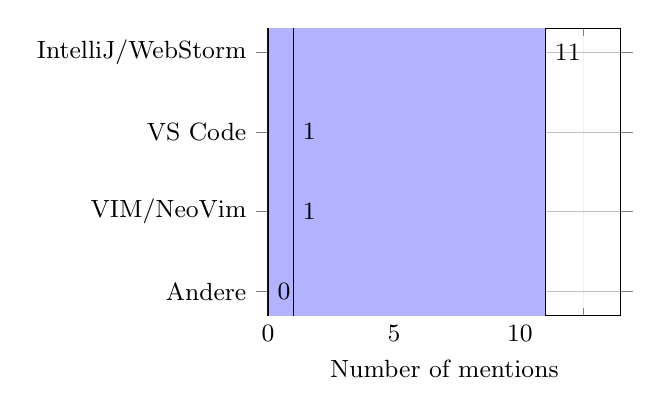
\begin{tikzpicture}
    \begin{axis}[
      width=\textwidth / 2,
      xbar,
      xmin=0,
      xmax=14,
      ticklabel style={font=\small},
      label style={font=\small},
      nodes near coords style={font=\small},
      bar width=20,
      nodes near coords,
      xlabel={Number of mentions},
      grid=both,
      grid style={line width=.1pt, draw=gray!10},
      major grid style={line width=.2pt,draw=gray!50},
      minor x tick num=1,
      ytick=data,
      yticklabels={IntelliJ/WebStorm, VS Code, VIM/NeoVim, Andere},
      ]
      \addplot[black,fill=blue!30!white] coordinates{ (11,4) (1,3) (1,2) (0,1) };
    \end{axis}
  \end{tikzpicture}
  \caption{Answers to question 15}
  \label{fig:app_usertest_q15}
\end{figure}
\subsection*{Question 16}
\label{sub:ut_q16}
Meine IDE hat mich während dem Usertest sinnvoll unterstützt. (Code Completion,
Inline Docs, Code Navigation,  Fehler/Warnungen)

\textit{Note:} This question allows us to determine if it is worth the effort
to write JSDoc.
\likertbarchart
  {Answers to question 16}
  {fig:app_usertest_q16}
  {10}{2}{1}{0}

\subsection*{Question 17}
\label{sub:ut_q17}
Das möchte ich sonst noch sagen:
\begin{table}[H]
  \centering
  \begin{tabularx}{\textwidth}{| X |} \hline
    Sehr detailliert und gut dokumentiert! \\ \hline 
    coole Idee, spannende Umsetzung. Die erste Aufgabe war recht anspruchsvoll ohne Repetition in eana. \\ \hline 
    Bei Fragen stehe ich gerne weiterhin zur Verfuegung.\\ \hline 
    Ich finde sehr sinvoll was ihr gemacht hab. Ich habe etwa 1.5 Stunden aufgewendet und konnte Einblicke in etwas bekommen, was ich so noch nicht kannte, danke dafür! \\ \hline
    Ich finde die Idee gut, man müsste die Errors besser machen können damit es Anklang finden könnte. Wenn ich anstatt "C++" einen Output von f(x) => g \_f(x) (so in der Art wars), ist das debuggen sehr schwer. \\ \hline
    Vielen Dank für die Möglichkeit, dabei zu sein! Es war super, mein Gehirn mal wieder ein bisschen zu quälen, äh, ich meine natürlich anzustrengen, durch die Tests. \\ \hline
    +Spannendes Projekt, dass praktische Funktionalität bringt, die man sich beispielsweise auch durch Lodash holen kann, aber vor allem erlaubt eure Implementation Entwicklern ihre eigenen Funktionen hinzuzufügen \\ \hline
    Tolle Arbeit! \\ \hline
    Cool! \\ \hline

  \end{tabularx}
  \caption{Answers to question 17}
  \label{tab:app_usertest_q17}
\end{table}
% section General Questions (end)
